\section{Гладкие многообразия}

\begin{definition}
	Пусть $X$ "--- топологическое пространство. \textit{Локальной картой} на $X$ называется пара $(U, \phi)$, где $U \subset X$ "--- непустое открытое множество, $\phi: \R^n \to U$ "--- \textit{гомеоморфизм}, то есть биекция такая, что $\phi$ и $\phi^{-1}$ непрерывны.
\end{definition}

\begin{note}
	Можно считать, что гомеоморфизм $\phi$ действует не на $\R^n$, а на открытом шаре $B_R(x_0) \subset \R^n$, поскольку между ними имеет место гомеоморфизм вида $x \mapsto x_0 + \frac R{|x| + 1}x$.
\end{note}

\begin{definition}
	\textit{Гладким $n$-мерным многообразием} называется хаусдорфово топологическое пространство $X$ с счетной базой и системой локальных карт $\{(U_\alpha, \phi_\alpha)\}_{\alpha \in \mf A}$, удовлетворяющей следующим условиям:
	\begin{enumerate}
		\item Для любого $\alpha \in \mf A$ гомеоморфизм $\phi_\alpha$ действует на $\R^n$
		\item $\bigcup_{\alpha \in \mf A}U_\alpha = X$
		\item Если для некоторых индексов $\alpha, \beta \in \mf A$ выполнено $U_\alpha \cap U_\beta = V \ne \emptyset$, то отображение $\phi_\beta^{-1} \circ \phi_\alpha : \phi_\alpha^{-1}(V) \to \phi_\beta^{-1}(V)$ является гладким
	\end{enumerate}
	
Число $n$ называется \textit{размерностью многообразия} и обозначается через $\dim{X}$.
\end{definition}

\begin{example}
	Покажем, что сфера $S^n = \{x \in \R^{n+1} : |x| = 1\}$ является гладким $n$-мерным многообразием с двумя картами. Сначала зададим одной картой множество $S^n \bs \{(1, 0, \dotsc, 0)^T\}$. Воспользуемся \textit{стереографической проекцией} на плоскость $x_0 = -1$. Произвольный вектор $(x_0, x) \in S^{n+1}$ при стереографической проекции переходит в вектор $y := \frac{2}{1-x_0}x \in \R^n$. Обратное преобразование имеет вид:
	\[y \mapsto \left(\frac{|y|^2 - 4}{|y|^2 + 4}, \frac{4}{y^2 + 4}y\right)\]
	
	Стереографическая проекция имеет наглядную геометрическую интерпретацию:
	\begin{center}
		\scalebox{1.2}{
		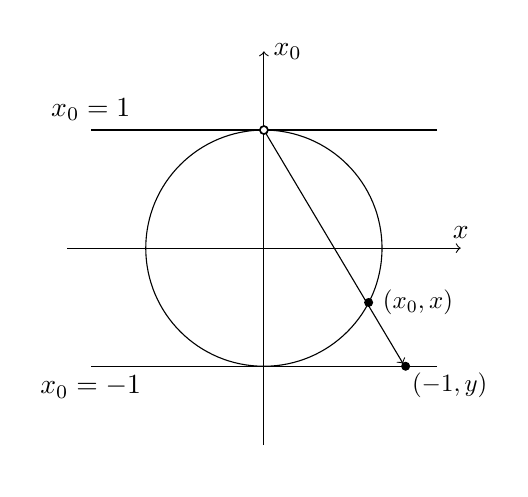
\begin{tikzpicture}
			\clip (-3, -2.8) rectangle (3, 2.8);
			\draw [->] (-2.5, 0) -- (2.5, 0) node [above, black] {$x$};
			\draw [->] (0, -2.5) -- (0, 2.5) node [right, black] {$x_0$};
			
			\draw (2.2, 1.5) -- (-2.2, 1.5) node [above] {$x_0 = 1$};
			\draw (2.2, -1.5) -- (-2.2, -1.5) node [below] {$x_0 = -1$};
			\draw[black] (0,0) circle[radius = 1.5]; 
			
			\node[draw, circle, inner sep=1.1pt, fill, black] at (0, 1.5) {};
			\draw [black, ->] (0, 1.5) -- (1.77, -1.47) node [black, below right, scale = 0.9] {$(-1, y)$};
			\node[draw, circle, inner sep=0.6pt, fill, white] at (0, 1.5) {};
			
			\node[draw, circle, inner sep=1pt, fill, black] at (1.8, -1.5) {};
			\node[draw, circle, inner sep=1pt, fill, black, label={right : \scalebox{0.9}{$(x_0, x)$}}] at (1.33, -0.69) {};
		\end{tikzpicture}}
	\end{center}
	
	Легко проверить, что стереографическая проекция на противоположную плоскость $x_0 = 1$ имеет вид $(x_0, x) \mapsto \frac2{1+x_0}x$ и задает множество $S^n \bs \{(-1, 0, \dotsc, 0)^T\}$. Две полученных карты удовлетворяют определению гладкого многообразия.
\end{example}

\begin{proposition}
	Любое открытое множество $G \subset \R^n$ со стандартной топологией является гладким $n$-мерным многообразием.
\end{proposition}

\begin{proof}
	Поскольку $G$ "--- открытое, то для любого $x \in G$ существует $R_x > 0$ такое, что $B_{R_x}(x) \subset G$. Тогда искомым набором локальных карт будет $\{(B_{R_x}(x), \id_{B_{R_x}(x)})\}$.
\end{proof}

\begin{definition}
	Пусть $X, Y$ "--- гладкие многообразия. \textit{Гладким отображением} между ними называется отображение $f: X \to Y$ такое, что для любых локальных карт $(U, \phi)$ на $X$ и $(V, \psi)$ на $Y$, для которых $f(U) \cap V \ne \emptyset$, отображение $\psi^{-1} \circ f \circ \phi$ является гладким на области определения.
\end{definition}

\begin{definition}
	\textit{Гладким путем} на гладком многообразии $X$ называется гладкое отображение $\gamma : [0, 1] \to X$.
\end{definition}

\begin{definition}
	Пусть $X$ "--- гладкое многообразие. Гладкие пути $\gamma_1, \gamma_2$ на $X$ с началом в точке $a \in X$ называются \textit{эквивалентными}, если для любой локальной карты $(U, \phi)$ на $X$ такой, что $a \in U$, выполнено $(\phi^{-1} \circ \gamma_1)'(0) = (\phi^{-1} \circ \gamma_2)'(0)$. Фактормножество гладких путей с началом в точке $a$ по этому отношению эквивалентности называется \textit{касательным пространством} к $X$ в точке $a$. Обозначение "--- $T_aX$.
\end{definition}

\begin{note}
	В определении эквивалентности гладких путей достаточно проверять равенство градиентов только для одной карты $(U, \phi)$, для которой $a \in U$. Действительно, если $\gamma$ "--- гладкий путь с началом в точке $a$, а $(V, \psi)$ "--- другая такая карта, то:
	\[(\psi^{-1} \circ \gamma)'(0) = \left((\psi^{-1} \circ \phi) \circ (\phi^{-1} \circ \gamma)\right)'(0) = (\psi^{-1} \circ \phi)'(\phi^{-1}(a))(\phi^{-1} \circ \gamma)'(0)\]
	
	Как видим, при переходе к другой карте градиенты меняются не зависящим от $\gamma$ образом. Отметим, что касательное пространство $T_aX$ при фиксированной локальной карте $(U, \phi)$ естественным образом отождествляется с $\R^{\dim{X}}$ сопоставлением $[\gamma] \mapsto (\psi^{-1} \circ \gamma)'(0)$. Сопоставление зависит от локальной карты, однако все полученные пространства являются канонически изоморфными.
\end{note}

\begin{proposition}
	Пусть $X, Y, Z$ "--- гладкие многообразия, и отображения $f : X \to Y$, $g : Y \to Z$ "--- гладкие. Тогда $g \circ f : X \to Z$ "--- тоже гладкое отображение.
\end{proposition}

\begin{proof}
	Зафиксируем $(U, \phi)$ и $(W, \theta)$ "--- такие локальные карты на $X$ и $Z$, что $g(f(U)) \cap W \ne \emptyset$. Выберем произвольную карту $(V, \psi)$ на $Y$, для которой $f(U) \cap V \ne \emptyset$. Тогда отображения $\psi^{-1} \circ f \circ \phi$ и $\theta^{-1} \circ g \circ \psi$ являются гладкими на области определения, поэтому и отображение $\theta^{-1} \circ g \circ f \circ \phi$ является гладким на области определения. В силу произвольности выбора карты $(V, \psi)$, получено требуемое.
\end{proof}

\begin{definition}
	Пусть $X, Y$ "--- гладкие многообразия, $f : X \to Y$ "--- гладкое отображение. \textit{Дифференциалом} отображения $f$ в точке $a \in X$ называется линейное отображение $d_af: T_aX \to T_{f(a)}Y$ вида $[\gamma] \mapsto [f \circ \gamma]$.
\end{definition}

\begin{proposition}
	Дифференциал $d_af$ гладкого отображения $f: X \to Y$ определен корректно и линеен.
\end{proposition}

\begin{proof}
	Зафиксируем локальные карты $(U, \phi)$ на $X$ и $(V, \psi)$ на $Y$ такие, что $a \in U$ и $f(a) \in V$. Рассмотрим произвольный гладкий путь $\gamma$ на $X$ с началом в точке $a$. Тогда:
	\[(\psi^{-1} \circ f \circ \gamma)'(0) = \left((\psi^{-1} \circ f \circ \phi) \circ (\phi^{-1} \circ \gamma)\right)'(0) = (\psi^{-1} \circ f \circ \phi)'(\phi^{-1}(a))(\phi^{-1} \circ \gamma)'(0)\]
	
	Поскольку значения $(\phi^{-1} \circ \gamma)'(0)$ в одном классе кривых $[\gamma] \in T_af$ одинаковы, то и значения $(\psi^{-1} \circ f \circ \gamma)'(0)$ для кривых этого класса одинаковы. Значит, определение корректно. Линейность полученного отображения также следует из равенства выше.
\end{proof}

\begin{note}
	При фиксированной локальной карте мы отождествляем касательное пространство с пространством $\R^{\dim{X}}$, поэтому можно считать, что дифференциал действует как линейное отображение $\R^{\dim{X}} \to \R^{\dim{Y}}$ с матрицей $(\psi^{-1} \circ f \circ \phi)'(\phi^{-1}(a))$.
\end{note}

\begin{proposition}
	Пусть $X, Y, Z$ "--- гладкие многообразия, и отображения $f : X \to Y$, $g : Y \to Z$ "--- гладкие. Тогда для каждой точки $a \in X$ выполнено $d_a(g\circ f) = d_{f(a)}g \circ d_af$.
\end{proposition}

\begin{proof}
	Зафиксируем локальные карты $(U, \phi)$ на $X$, $(V, \psi)$ на $Y$ и $(W, \theta)$ на $Z$ такие, что $a \in U$, $f(a) \in V$ и $g(f(a)) \in W$. Достаточно проверить, что преобразование градиентов дифференциалами производится так, как в условии:
	\begin{multline*}
		(\theta^{-1}\circ g \circ f \circ \phi)'(\phi^-1(a)) = \left((\theta^{-1}\circ g \circ \psi) \circ (\psi^{-1} \circ f \circ \phi)\right)'(\phi^-1(a)) = \\
		=(\theta^{-1}\circ g \circ \psi)'\left(\psi^{-1}(f(a))\right)(\psi^{-1} \circ f \circ \phi)'(\phi^{-1}(a))
	\end{multline*}
	
	Таким образом, получено требуемое.
\end{proof}